\documentclass{article}

% package imports
%\usepackage[top=1in, bottom=1in, left=1in, right=1in]{geometry} 
\usepackage{hyperref} 
\usepackage[utf8]{inputenc}
\usepackage{graphicx}
\usepackage{amsmath}
\usepackage{amsthm}
\usepackage{amssymb}
\usepackage{complexity}


\newtheorem{theorem}{Theorem}[section]
\newtheorem{lemma}{Lemma}[section]
\theoremstyle{definition} 
\newtheorem{definition}{Definition}[section]

\newcommand{\plain}[1]{\,\text{#1}\,}
\newcommand{\sigmastar}{\Sigma^{*}}
\newcommand{\kr}{\leq^{p}_{ker}}

% define the author, title, and date
\author{Jeffrey Finkelstein} 
\date{May 2010} 
\title{Untitled}

\begin{document}

\maketitle

\section{Definitions}

In the following definitions, $x,y,a\in{\Sigma^*}$.

Let $R_{par}=\{(x,y)|x \plain{and} y \plain{have the same parity}\}$.

Let $R_{bc}=\{(x,y)|x \plain{and} y \plain{have the same number of ones}\}$.

Let $R_{eq}=\{(x,y)|x = y\}$.

Let $R_{eqi}=\{(x,y)|x = y \lor x = \bar{y}\}$.

Let $R_{a}=\{((a,x),(a,y))|x = y \lor x \oplus y = a\}$. ($R_{a}$ is a family
of equivalence relations; $R_{a}$ is a different relation for each fixed $a\in\sigmastar$.)

Notice the following equivalent definitions, where $n$=$|x|$=$|y|$:
$R_{eq}=\{(x,y)|x \oplus y = 0^n\}$, $R_{eqi}=\{(x,y)|x \oplus y = 0^n \lor x
\oplus y = 1^n\}$, and $R_{a}=\{((a,x),(a,y))|x \oplus y = 0^n \lor x \oplus
y\ = a\}$.

Let $GI=\{(G_1,G_2)|G_1 \plain{and} G_2 \plain{are undirected graphs and} G_1
\plain{is isomorphic to} G_2\}$.

\begin{definition}Let $R,S\subseteq\sigmastar\times\sigmastar$. We say $R$
  \textit{kernel reduces to} $S$ if $\exists f\in\FP:\forall x,y\in\sigmastar
  (x,y)\in R \leftrightarrow (f(x),f(y))\in S$. We denote this by $R\kr
  S$.\end{definition}

\section{Relationships among equivalence relations}
%% TODO show that all the stated equivalence relations are actually eq. rel.s

\begin{theorem}$R_{eq} \subsetneq R_{bc} \subsetneq R_{par}$\end{theorem}
\begin{proof}
  Let $(x,y)\in R_{eq}$, so $x=y$. Then $x$ has exactly the same number of ones
  as $y$ (and the same number of zeros, and in the same order), so $(x,y) \in
  R_{bc}$. Therefore, $R_{eq} \subset R_{bc}$.
 
  Consider $x=1100$ and $y=0101$. Then $(x,y)\in R_{bc}$ but $(x,y) \notin
  R_{eq}$. Therefore $R_{eq} \neq R_{bc}$.

  Let $(x,y)\in R_{bc}$, so $x$ and $y$ have the same number of ones. Let $k$
  be the number of ones in $x$, and $l$ be the number of ones in $y$. Then
  $l=k$, which implies $l \equiv k (mod 2)$. Therefore $x$ and $y$ have the
  same parity, so $(x,y)\in R_{par}$. Therefore $R_{bc} \subset R_{par}$.

  Consider $x=1000$ and $y=1011$. Then $(x,y)\in R_{par}$ but $(x,y) \notin
  R_{bc}$. Therefore $R_{bc} \neq R_{par}$.
\end{proof}

\begin{theorem}$R_{eq} \subsetneq R_{eqi}$\end{theorem}
\begin{proof}
  Let $(x,y)\in R_{eq}$, so $x=y$. Then $(x,y)$ satisfies the property
  specified in the definition of $R_{eqi}$, specifically that $x=y$, so
  $(x,y) \in R_{eqi}$. Therefore $R_{eq} \subset R_{eqi}$.

  Consider $x=1000$ and $y=0111$. Then $(x,y)\in R_{eqi}$ but $(x,y) \notin
  R_{eq}$. Therefore $R_{eq} \neq R_{eqi}$.
\end{proof}

Figure \ref{fig:containments} exhibits the containments among $R_{eq}$,
$R_{eqi}$, $R_{bc}$, and $R_{par}$. Note that if $a=0^n$, for $n=|x|=|y|$, then
$R_{a}=R_{eq}$, and if $a=1^n$ then $R_{a}=R_{eqi}$.

%% \begin{lemma}Let $R,S \subseteq \sigmastar\times\sigmastar$ be two
%%   equivalence relations. If $R\subseteq S$ then $R\leq^{p}_{ker}S$.\end{lemma}
%% \begin{proof}
%%   Consider the identity function, $I:\sigmastar\to\sigmastar$, defined by
%%   $I(w)=w, \forall w\in\sigmastar$. Suppose $(x,y)\in R$. Then
%%   $(I(x),I(y))=(x,y)\in R \subseteq S$. Suppose $(x,y) \notin R$. Then
%%   $(I(x),I(y))=(x,y)\notin R \subseteq S$. Therefore $(x,y)\in R
%%   \leftrightarrow (I(x),I(y))\in S$, that is, $R \leq^{p}_{ker}S$.
%% \end{proof}

\begin{figure}
  \begin{center}
    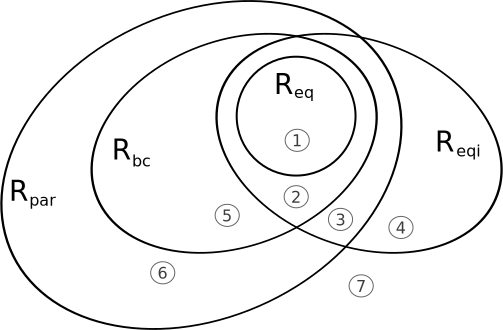
\includegraphics[width=300px,height=241px,keepaspectratio=true]
                    {containments.png}
  \end{center}
  \caption{ \label{fig:containments} Containment relationships for equivalence
    relations $R_{eq}$, $R_{eqi}$, $R_{bc}$, and $R_{par}$. The following are
    example elements in the sets at the specified locations: 1. (1100, 1100)
    2. (1010, 0101) 3. (1000, 0111) 4. (10000, 01111) 5. (1000, 0001) 6. (1000,
    1011) 7. (1000, 0000) }
\end{figure}

\section{Results}

\begin{theorem}$R_{par}\kr GI$\end{theorem}
\begin{proof}
  Construct $M\in FP$ on input $w\in\sigmastar$:
  \begin{enumerate}
  \item Initialize set of vertices $V_w=\{v_{p}, v_{o}\}$ and set of
    (undirected) edges $E_w=\{\}$.
  \item for $i=1$ to $|w|$:
    \begin{enumerate}
    \item If $w_i=1$ and $(v_{o}, v_{p})\notin E_w$, add undirected edge
      $(v_{o}, v_{p})$ to $E_w$.
    \item Else if $w_i=1$ and $(v_{o}, v_{p})\in E_w$, remove $(v_{o}, v_{p})$
      from $E_w$.
    \end{enumerate}
  \item Output $G_w=(V_w,E_w)$.
  \end{enumerate}

  Suppose $(x,y)\in R_{par}$, so either $x$ and $y$ both have even parity or
  $x$ and $y$ both have odd parity. 

  If $x$ and $y$ both have even parity, $x$ contains $2k$ ones and $y$ contains
  $2l$ ones, for some $k,l\in\mathbb{N}$. Since $2k$ is even, machine $M$ on
  input $x$ adds then removes the edge $(v_o, v_p)$ to and from $E_x$ an equal
  number of times. Similarly for $M$ on input $y$. Therefore $M(x)$ outputs
  $G_x=(V_x, E_x)$, where $V_x=\{v_o, v_p\}$ and $E_x=\{\}$, and $M(y)$ outputs
  $G_y=(V_y, E_y)$, where $V_y=\{v_o, v_p\}$ and $E_y=\{\}$. Then $G_x$ is
  isomorphic to $G_y$ by the identity function, $I:V_x\to V_y$, defined by
  $I(v)=v, \forall v\in V_x$.

  If $x$ and $y$ both have odd parity, $x$ contains $2k+1$ ones and $y$
  contains $2l+1$ ones, for some $k,l\in\mathbb{N}$. Since $2k+1$ is odd,
  machine $M$ on input $x$ adds edge $(v_o, v_p)$ to $E_x$ one more time than
  it removes the edge. Similarly for $M$ on input $y$. Therefore $M(x)$ outputs
  $G_x=(V_x, E_x)$, where $V_x=\{v_o, v_p\}$ and $E_x=\{(v_o, v_p)\}$, and
  $M(y)$ outputs $G_y=(V_y, E_y)$, where $V_y=\{v_o, v_p\}$ and $E_y=\{(v_o,
  v_p)\}$. Then $G_x$ is isomorphic to $G_y$ by the identity function,
  $I:V_x\to V_y$, defined by $I(v)=v, \forall v\in V_x$.

  Suppose $(x,y)\notin R_{par}$, so without loss of generality, $x$ has even
  parity and $y$ has odd parity. Then $x$ contains $2k$ ones and $y$ contains
  $2l+1$ ones, for some $k,l\in\mathbb{N}$. Since $2k$ is even, machine $M$ on
  input $x$ adds then removes the edge $(v_o, v_p)$ to and from $E_x$ an equal
  number of times. Since $2l+1$ is odd, machine $M$ on input $y$ adds edge
  $(v_o, v_p)$ to $E_y$ one more time than it removes the edge. Therefore
  $M(x)$ outputs $G_x=(V_x, E_x)$, where $V_x=\{v_o, v_p\}$ and $E_x=\{\}$, and
  $M(y)$ outputs $G_y=(V_y, E_y)$, where $V_y=\{v_o, v_p\}$ and $E_y=\{(v_o,
  v_p)\}$. Since $(v_o, v_p)\in E_y$ but $(v_o, v_p)\notin E_x$, so no
  bijection exists between $V_x$ and $V_y$ which preserves edges. Therefore,
  $G_x$ is not isomorphic to $G_y$.

  Since $(x,y)\in R_{par} \leftrightarrow (M(x), M(y)) \in GI$, we have shown
  $R_{par} \kr GI$.
\end{proof}

\begin{theorem}$R_{bc}\kr GI$\end{theorem}
\begin{proof}
  
  %% TODO this fails for 1110 and 0111; 
  %% need to add a triangle structure onto v_one
  Construct $M\in FP$ on input $w \in \sigmastar$:
  \begin{enumerate}
  \item Initialize set of vertices $V_w=\{v_{zero}, v_{one}\}$ and set of
    (undirected) edges $E_w=\{\}$.
  \item for $i=1$ to $|w|$:
    \begin{enumerate}
    \item Add $v_i$ to $V_w$.
    \item If $w_i = 1$, add undirected edge $(v_i, v_{one})$ to $E_w$.
    \item Else if $w_i = 0$, add undirected edge $(v_i, v_{zero})$ to $E_w$.
    \end{enumerate}
  \item Output $G_w=(V_w,E_w)$.
  \end{enumerate}
  
  Suppose $(x,y)\in R_{bc}$, so $x$ and $y$ have the same number of ones, say
  $k\in\mathbb{N}$. Assume $|x|=|y|=n$, so both $x$ and $y$ have $n-k$
  zeros. Define $E_{w,1}=\{(v_i, v_{one})|v_i = 1\}$ and $E_{w,0}=\{(v_i,
  v_{zero})|v_i = 0\}$, so $E_x = E_{x,1}\cup E_{x,0}$ and $E_y = E_{y,1} \cup
  E_{y,0}$ by construction. Define $V_{w,b}=\{v_i|x_i=b\}$, so $V_x=V_{x,1}
  \cup V_{x,0}$ and $V_y=V_{y,1} \cup V_{y,0}$. Note that
  $|V_{x,1}|=|V_{y,1}|=k$ and $|V_{x,0}|=|V_{y,0}|=n-k$. Since
  $|V_{x,1}|=|V_{y,1}|=k$, there exists a bijection between them, call it
  $\phi_1:V_{x,1}\to V_{y,1}$. Similarly, since $|V_{x,0}|=|V_{y,0}|=k$, there
  exists a bijection between them, call it $\phi_0:V_{x,0}\to V_{y,0}$. Define
  $\phi:V_x\to V_y$ by 
  \begin{displaymath}
    \phi(v) = 
    \begin{cases}
      \phi_0(v) & \plain{if} v = 0\\
      \phi_1(v) & \plain{if} v = 1\\
      v & \plain{if} v = v_{zero} \plain{or} v = v_{one}
    \end{cases}
  \end{displaymath}
  for all $v\in V_x$.

  Since the only edges in $E_x$ are the edges $(v_i, v_{one})$ when $x_i=1$ and
  $(v_i, v_{zero})$ when $x_i=0$, then $(v_i, v_{one})\in V_x \leftrightarrow
  (\phi(v_i), \phi(v_{one}))=(\phi_1(v_i), v_{one})\in V_y$, and $(v_i,
  v_{zero})\in V_x \leftrightarrow (\phi(v_i), \phi(v_{zero})) = (\phi_0(v_i),
  v_{zero})\in V_y$. Therefore $\phi$ describes a graph isomorphism, so $G_1$
  is isomorphic to $G_2$.
  
  Suppose $(x,y)\notin R_{bc}$, so $x$ and $y$ have a different number of
  ones. Let $k$ be the number of ones in $x$, and $l$ be the number of ones in
  $y$, with $k\neq l$. Define $E_{w,0}$ and $E_{w,1}$ as above. Now
  $|E_{x,1}|=k$ and $|E_{y,1}|=l$. Since $k=|E_{x,1}|\neq|E_{y,1}|=l$, no
  bijection exists between them. 
\end{proof}

\end{document}
